\documentclass[11pt]{article}

% Remove the "review" option to generate the final version.
\usepackage{naacl2021}

% Standard package includes
\usepackage{times}
\usepackage{latexsym}
\usepackage[T1]{fontenc}
\usepackage[utf8]{inputenc}
\usepackage{microtype}
\usepackage{graphicx}
\usepackage{booktabs}
\usepackage{amsmath}

% If the title and author information does not fit in the area allocated, uncomment the following
%
%\setlength\titlebox{<dim>}
%
% and set <dim> to something 5cm or larger.

\title{\textbf{Understanding Flight Delays}\\\textbf{CSE 519: Data Science Fundamentals}\\\textbf{Project Final Report}}
%\author{
%  Kai Li \\
%  \texttt{kai.li@stonybrook.edu} \\\And
%  Peng Fei Yao \\
%  \texttt{pengfei.yao@stonybrook.edu} \\
%}

\begin{document}
\maketitle
\begin{abstract}
Airline flight delay is one of the most pressing and prominent problems in the world due to its prevalent impact on human society in the 21st century. We use data from the U.S. Department of Transportation (DOT) Bureau of Transportation Statistics (BTS) to obtain a comprehensive record of airline information, airport information, and flight delay statistics. This project concerns the impact of flight delays on airports and airlines, both numerically and graphically. We are also devoted to investigating the potential factors that have a connection with flight delays so that remedial measures can target those relationships. Additionally, modeling the total time (minutes) of delayed flights under given conditions is beneficial for the decision makers for the logistics of the airport when they lack information on the total minutes of delayed flights due to specific causes. Finally, decision makers can also apply machine learning models for prediction purposes.
\end{abstract}

\section{Introduction}\label{sec:intro}
Commercial air travel is one of the most welcoming forms of travel from one place to another due to its quicker speed, convenience, and safety. Statistics from \citet{web:statista} show that the number of passengers using air transport keeps increasing every year from 2004 to 2019. Specifically speaking, the \citet{web:faa1} (FAA) reported that more than 10 million passenger flights were scheduled in 2019. On the other hand, BTS also releases data on flights arrival performance by four types of flight status every year. Specifically, from January 2012 to December 2019, 79.54 percent of operating carrier flights are on-time; 18.63 percent are delayed; 1.58 percent are canceled; and 0.24 percent are diverted \citep{web:bts1}. In general, FAA and BTS consider a flight delayed if the actual arrival time at the airport gate is 15 minutes or more later than the scheduled arrival time recorded in the Computerized Reservation System (CRS). Otherwise, the arrival flight is considered on-time. What is more, the possible delay reasons are air carrier, weather, National Aviation System (NAS), security, or a previous flight using the same aircraft being late, according to FAA and BTS.

Among the 18.63 percent delays, BTS also specifies the reasons for the delay causes\footnote{Note that it is possible to have multiple delays causes assigned to one delayed flight.}. In most cases, flight delays are due to air carrier delay, NAS delay, and aircraft arriving late delay with respective probabilities of 28.61 percent, 30.92 percent, and 37.25 percent. The chances of delays due to weather and security are only 3.06 percent and 0.16 percent. 

From another angle, Figure \ref{fig:bar_plot1} presents the average delay rate by year from 2012 to 2019. We notice that the difference between the highest delay rate in 2014 and the lowest delay rate in 2016 is about 5 percent, which is significant in our opinion. Furthermore, the delay rate has not been decreasing, which may indicate that existing strategies to deal with flight delays may not be very successful in reducing the delay rate. 

\begin{figure}[h!]
\centering
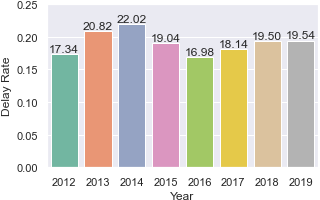
\includegraphics[width = \columnwidth]{bar_plot1}
\caption{On-Time Arrival Performance By Year (in Percentage)}\label{fig:bar_plot1}
\end{figure}

Researchers also spent a lot of time investigating the consequences and solutions to flight delays due to their vast connections to other subjects. In particular, research has shown that flight delays have profound effects on aviation, passengers, airports, airlines, and the United States economy \citep{ar:carvalho_et_al, ar:peterson_neels_barczi_graham}. For example, flight delays impact the schedules of airlines and airports in landing, take-off, ground activities, supplies, and so on; the time travelers spent on unwanted waiting creates anxiety and concerns that reduce business productivity and passengers' active leisure \citep{ar:peterson_neels_barczi_graham}; from economic welfare's perspective, \citet{ar:britto_dresner_voltes} claim that every traveler can earn about 1.5 to 2.5 dollars from a 10 percent reduction in delays. Hence, a more thorough understanding of flight delays is urgent to minimize the negative impacts. 

In addition to the existing research done on flight delays, we realize the importance of additional characteristics of airlines and airports, besides the ones provided in regular flight delay data. Especially, the primary flight delay sources only contain basic information such as the date, airline/airport name, and delays causes statistics. We are also interested in other factors that potentially have a relation to flight delays. For example, we believe carriers with larger market sizes tend to have lower delay rates from our air-traveling experience. To verify this, we need a set of standards to define market size. Another guess is that the busiest airports are more likely to have higher delay rates compared to others. Again, we need classification to categorize the existing airports into the busiest airports and less busy airports to continue with the analysis.

Another important objective for this project is model building. Due to the complexity of the commercial transportation system, we believe that decision makers can encounter a variety of unforeseen scenarios, such as predictions while important data is missing. Thus, modeling the total time (minutes) of delayed flights under given conditions is critical to help with the aviation decision-making process.

The remainder of the paper is organized as follows: Section \ref{sec:data} gives an overview of the datasets used in this paper to analyze flight delays and machine learning model formulation. Section \ref{sec:methods} gives a more detailed methodology for exploratory data analysis and modeling using the preprocessed complete dataset. Section \ref{sec:results} provides detailed results of the analysis and model evaluation. Section \ref{sec:discussion} concludes the project and provides additional comments with future research directions.

\section{Datasets}\label{sec:data}
For this project, we use five datasets sourced from the BTS databases. Before discussing each dataset, we provide basic summary information for the datasets. The main dataset contains 123,896 total records with comprehensive information on airlines, airports, and flight delay statistics from January 2012 to December 2019 in the United States. After a preliminary data exploration, we observe 156 missing values in the number of arrival flights delayed in the dataset. Interestingly, we notice that the missing values are not missing entirely at random. 135 of the missing values are also missing in all of the flight delay statistics. The rest of the 21 missing value observations have no arrival flights delayed. Thus, to properly handle the missing values, we first delete the 135 missing values due to the record missing entirely. Then, we impute the 21 missing values by 0 to correctly record the number of arrival flights delayed. The rest of the four secondary datasets are preprocessed already by filtering relevant useful data from their respective BTS databases. We finish data preprocessing by merging the five datasets by primary keys to obtain the complete dataset. Additional details for the datasets are provided in each subsection.

\subsection{Airline On-Time Arrival Performance Data}
Airline On-Time Arrival Performance Dataset is the primary dataset from the BTS database of Airline On-Time Statistics and Delay Causes \citep{web:bts2}. It contains 21 variables documenting the necessary information to investigate the elementary relationships between flight delays statistics and basic aviation information. Variable descriptions are given below.

\begin{description}
\item [Date] Year and month.
\item [Airline Information] Airline code and name.
\item [Airport Information] Airport code and name.
\item [On-Time Statistics] Number of flights which arrived at the airport; number of flights delayed; number of canceled flights; number of diverted flights; and total time (minutes) of delayed flights.
\item [Delay Causes Statistics] Number of flights delayed and total time (minutes) of delayed flights due to air carrier, weather, National Aviation System (NAS), security, or a previous flight using the same aircraft being late.
\item [Derived Variables] Number of flights on-time (subtracting the number of flights delayed, canceled and diverted flights from the total number of arrival flights) and delay rate (ratio of number of flights delayed to number of flights which arrived at the airport).
\end{description}

\subsection{Airport Busyness Data}
Airport Busyness Data is a preprocessed secondary dataset from the BTS Airline On-Time Statistics and Delay Causes dataset \citep{web:bts2}. All airports have a unique name and code. That is, all airport names and airport codes are matched. Among the 375 airports in the dataset, 30 major airports, considered in BTS databases, will be classified as the busiest airports. The airport codes for the 30 major airports are ATL, BWI, BOS, CLT, MDW, ORD, DFW, DEN, DTW, FLL, HNL, IAH, LAS, LAX, MIA, MSP, JFK, LGA, EWR, MCO, PHL, PHX, PDX, SLC, SAN, SFO, SEA, TPA, DCA and IAD, in alphabetical order of airport names. A binary variable is sufficient to record if the airport is one of the busiest airports.

\begin{description}
\item [Airport Information] Airport code and name.
\item [Airport Busyness Information] Indicates if the airport is considered the busiest airport: 1 if busiest, and 0 otherwise.
\end{description}

\subsection{Airline Carrier Group Data}\label{sec:acgd}
Airline Carrier Group Data is another preprocessed secondary dataset from the BTS Aviation Support Tables database \citep{web:bts3}. Note that there are 20 airline codes and 23 airline names from January 2012 to December 2019. For example, airline code 9E corresponds to Pinnacle Airlines Inc. from 2002 to 2013 and Endeavor Air Inc. since 2013. In fact, Pinnacle Airlines Inc. bankrupted in 2013 and emerged again in 2013 under the name Endeavor Air Inc.. Similar situations happened to the other two carriers based on our research. In this project, we regard the 20 airline codes as the only official information about air carriers. That is, we combine carriers sharing the same code due to the nature of the International Air Transport Association (IATA) coding standards. 

There are, in total, nine carrier groups categorized by BTS based on the
airline’s carrier type and market size. After preprocessing the data, we find that all carriers on the list fall into either one of the two categories: national carrier and major carrier. \citet{web:bts3} defines national carriers and major carriers to be airlines with annual revenue of over \$100 million to \$1 billion and airlines with annual revenue of over \$1 billion, respectively.

\begin{description}
\item [Airline Information] Airline code.
\item [Carrier Group Information] Indicates the airline's carrier group: 2 if national carrier, and 3 if major carrier.
\end{description}

\subsection{Airline Marketing Carrier Data}
A different grouping of airlines is based on whether an airline is a marketing carrier. We have the Airline Marketing Carrier Data, an auxiliary dataset preprocessed from the BTS Air Carrier Statistics \citep{web:bts4}. The definition of a marketing carrier is tied to the Codeshare Agreement. Codeshare Agreement is a commercial agreement between air carriers that allows a marketing airline to put its two-letter identification code on the flights of another operating carrier as they appear in CRS \citep{web:bts3}. If an airline is a marketing carrier, carriers have their own market flights and regional codeshare partners. That is, they have a Codeshare Agreement. Otherwise, it is a regular carrier.

\begin{description}
\item [Airline Information] Airline code.
\item [Market Carrier Information] Indicates if the airline is a marketing carrier: 1 if marketing carrier, and 0 if regular carrier. 
\end{description}

\subsection{Airline Carrier History Data}\label{sec:hist}
Lastly, Airline Carrier History Data contains the start year and the end year of the establishment of airlines, preprocessed from the BTS Air Carrier Statistics \citep{web:bts4}. Note that the null values in the data mean that the associate carriers are still in operation, instead of the value being missing for any reason. We derive a new variable, time of establishment, calculated by the lag difference between the year of end and start. If the airline company is still open, we consider the end year as the current year 2021.

\begin{description}
\item [Airline Information] Airline code.
\item [Carrier History Information] Year of the start and year of the closure.
\item [Derived Variable] Years of establishment
\end{description}

\section{Methods}\label{sec:methods}
We use Python to perform all sets of data science procedures in this paper. For example, \texttt{pandas} and \texttt{NumPy} libraries are necessary to deal with data cleaning and scientific computing. We can join the primary and secondary datasets using the above libraries. Moreover, visualization is indispensable with libraries \texttt{Matplotlib} and \texttt{seaborn}. Figure \ref{fig:bar_plot1} in Section \ref{sec:intro} is created with the two libraries so that we can quickly identify the pattern and understand the story behind the plots easily. Graphical displays are consistently used to obtain creative insights throughout the paper.

Classical machine learning methods for data science and statistical procedures are provided in libraries \texttt{scikit-learn} and \texttt{SciPy}. We first build a baseline model, using multiple linear regression, based on our initial guess on the correlated factors. After obtaining sufficient understanding from the baseline, we move on to build more sophisticated machine learning models and evaluate their effectiveness in prediction. The scoring metrics used to evaluate model appropriateness require additional background research such that easy and interpretable results can be formed.

During the stage of model building, we will perform a series of model improvement analysis processes. For example, feature selection filters the features that contribute most to the prediction variable. We run feature selection by choosing the best $k$ regressors using the automated processes in Python, using a regression metric for evaluation. Then, feature engineering techniques are tried if needed to extract information to the largest extent from the raw data. Note that missing values manipulation, a kind of feature engineering, has been done in Section \ref{sec:data}. Hyperparameter tuning is utilized to obtain the optimal result among all models in the particular machine learning models. Especially, a randomized search is an automated procedure that tests different hyperparameters and outputs the best combination of hyperparameters using a suitable scoring metric. During the process of hyperparameter tuning, cross-validation is used to score the predictive models. In particular, we prefer a $k$-fold cross-validation.

Finally, we want to predict the total minutes of flight delays to ensure the models are good enough to be applied to real data. We use the main dataset Airline On-Time Arrival Performance Dataset again. However, the January 2020 data is used as our prediction dataset. Additionally, we shall provide two-sample t-tests for examining the differences between the predictions between each model. Note that the two independent samples t-test requires knowing if the variances of the two populations are the same. This assumption determines the hyperparameter setting in the t-test function in Python. Hence, we test the assumption for the two populations using a robust Levene’s test. If the test is significant, we conclude the variances of the two populations are not the same. Otherwise, we believe they are equal.

\section{Results}\label{sec:results}
In this section, we provide the graphical and numerical analysis using the methodologies introduced in Section \ref{sec:methods}. Section \ref{sec:seasonal} presents several important general results. These results enable us to understand the graphical analysis results in Sections \ref{sec:busy}, \ref{sec:market} and \ref{sec:estab} more comprehensively.

\subsection{Seasonal Effects on Flight Delay Rates}\label{sec:seasonal}
In our opinion, seasonal variations happen to the demand for air transport. For example, we observe more crowds of people at airports during the summer compared to school days, which may possibly increase the chance of flight delays. That is, seasonal effects may also correlate with variables of interest in this project. To verify this, we plot the average delay rate for each month by each year to observe if any seasonal trend occurs, as shown in Figure \ref{fig:line_plot1}. Based on our observation, there is an obvious pattern of mean delay rates from 2012 to 2019. In particular, delay rates in January start approximately at the medium level of all ranges of delay rates. Then, the curves move down generally until April. Next, delay rates start increasing and reach their peak in June and July. After that, the curves move downward again for the next three months. Finally, delay rates rise in November and reach another peak again in December. \citet{web:bts5} provides additional comments illustrating that transportation data tend to be highly seasonal.

\begin{figure}[h!]
\centering
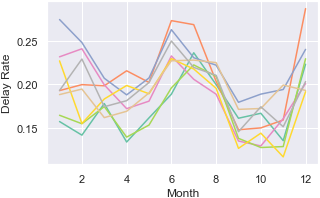
\includegraphics[width = \columnwidth]{line_plot1}
\caption{Delay Rate Season Effects for each Month Grouped by Year}\label{fig:line_plot1}
\end{figure}

\subsection{Delays in Busiest Airports and the others}\label{sec:busy}
Flight delays seem to be seasonal-variant. Are there any seasonality issues with different types of airports? The question can be answered by plotting the mean delay rate for each month, instead of the average delay rate for each year. The plot for the delay rate categorized by airport busyness is shown in Figure \ref{fig:line_plot2}. The plot shows the same trend discussed in Section \ref{sec:seasonal} for both types of airports. Hence, the seasonality of delay rates also holds among the airports.

\begin{figure}[h!]
\centering
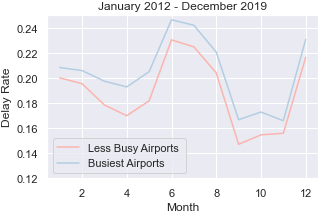
\includegraphics[width = \columnwidth]{line_plot2}
\caption{Busiest vs. Less Busy Airports On-Time Arrival Performance by Month}\label{fig:line_plot2}
\end{figure}

Furthermore, we are also interested in whether busiest airports tend to have higher delay rates than less busy airports, as discussed in our motivation example in Section \ref{sec:intro}. Figure \ref{fig:line_plot2} presents an immediate result that the busiest airports have higher delay rates at any time than the other airports. The average difference between the delay rates is approximately 1.63 percent.

\subsection{Delays Versus Airline Market Size}\label{sec:market}
After discovering the relationship between airports and flight delay rates, it is natural to consider if different classifications of airline carriers can impact flight delay rates. However, airline classification is more complicated than airport classification due to the complexity of the airline structure. Therefore, we first present some general airline information on flight delays. Figure \ref{fig:bar_plot2} reveals the delay rate for the 20 airlines in the data. The carrier with airline code HA (Hawaiian Airlines Inc.) has the lowest mean delay rate from 2012 to 2019, while the airline F9 (Frontier Airlines Inc.) has the highest. Numerically, the mean delay rates for Hawaiian Airlines Inc. and Frontier Airlines Inc. are 9.32 percent and 24.61 percent, respectively. We are curious why the difference in delay rates can vary so much. Additional details are discussed in Section \ref{sec:discussion}.

\begin{figure}[h!]
\centering
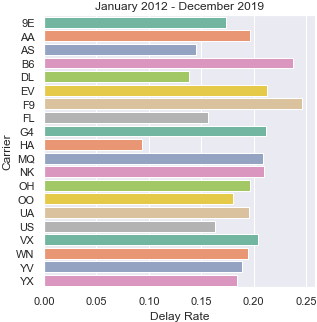
\includegraphics[width = \columnwidth]{bar_plot2}
\caption{Airlines On-Time Arrival Performance}\label{fig:bar_plot2}
\end{figure}

Similarly, we graph the following delay rates for each airline carrier group in terms of months to check if airlines also exhibit seasonal trends. The graph is shown in Figure \ref{fig:line_plot3}. Note that seasonal variation persists for two carrier groups.

\begin{figure}[h!]
\centering
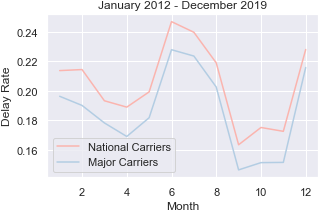
\includegraphics[width = \columnwidth]{line_plot3}
\caption{National vs. Major Carriers On-Time Arrival Performance by Month}\label{fig:line_plot3}
\end{figure}

We care about whether airlines with larger market size are more likely to have lower delay rates. Figure \ref{fig:line_plot3} concludes that national carriers have higher delay rates from 2012 to 2019 for all months. The average difference is about 1.84 percent.

Another classification for airlines is whether they are marketing carriers. Figure \ref{fig:line_plot4} shows no uniform pattern. For example, regular carriers tend to have lower delay rates in June and July, but higher delay rates at other times. Thus, further analysis is needed, as discussed in Section \ref{sec:discussion}. 

\begin{figure}[h!]
\centering
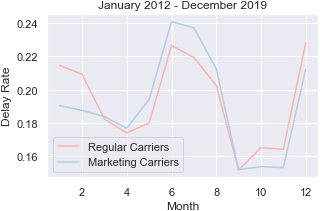
\includegraphics[width = \columnwidth]{line_plot4}
\caption{Regular vs. Marketing Carriers On-Time Arrival Performance by Month}\label{fig:line_plot4}
\end{figure}

\subsection{Delays Versus Airline Establishment Time}\label{sec:estab}
We want to see the relationship between flight delays and airline establishment time. It is difficult to model the relationship due to the bankruptcy and reoperation of airlines. As stated in Section \ref{sec:hist}, we treat the special cases of different airlines sharing the same code as combined entities. For example, Pinnacle Airlines Inc., with airline code 9E, started in 2002 and ended in 2013; Endeavor Air Inc. emerged with the same airline code 9E in 2013. Hence, we consider the start of the establishment as 2002, instead of 2013. The regression plot for delay rate versus years of establishment is provided in Figure \ref{fig:reg_plot}. A regression line with a 95 percent confidence interval is provided. Note that the regression line is nearly horizontal, which indicates that the years of the establishment may be independent of the delay rate. In particular, we observe carriers with about 60 years of establishment have average delay rates that vary from about 14 percent to 25 percent. Therefore, years of establishment may not be a useful variable. 

\begin{figure}[h!]
\centering
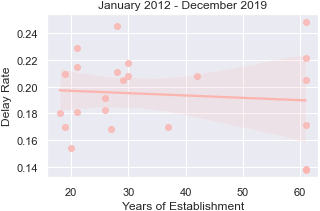
\includegraphics[width = \columnwidth]{reg_plot}
\caption{Delay Rate by Years of Establishment}\label{fig:reg_plot}
\end{figure}

\subsection{Modeling and Prediction}
Modeling and prediction are critical to finding the best solution under given scenarios. We provide the results for model building and prediction based on the methods discussed in Section \ref{sec:methods}.

\subsubsection{Baseline Model}
To begin with the modeling building process, we start with a baseline model. We consider using a multiple linear regression model as the baseline because of its quick learning process and simplicity in code implementation. In terms of the simple features for the baseline, we choose the correlated features based on our common knowledge. In particular, variables month, whether the airport is among the busiest, and carrier group are considered as the regressors with the total minutes of flight delayed as the dependent variable. Lastly, we train the baseline model with  default hyperparameters. The performance result is shown in Section \ref{sec:performance}.

\subsubsection{Feature Selection and Engineering}
In this project, we believe that selecting five regressors is sufficient for feature selection. Before implementing the selection algorithm, we notice that airport code/name and airline code/name cannot be used in regression models directly since they are categorical. Feature engineering techniques can be used to address the issue. We use a one-hot encoding scheme to create binary columns for each category of airport and airline code. We do not have to create binary columns for airport and airline names because they contain the same imformation in the data. Additionally, we are alerted that the response variable, the total minutes of delayed flights, can be calculated by the sum of the total time of delayed flights due to the five delay causes. It is not meaningful to build machine learning models given a specified linear relationship. Hence, we delete the five directly related variables in the feature selection process. The five most active features are number of flights that arrived at the airport, number of flights delayed, number of flights delayed due to air carrier, NAS and late aircraft.

\subsubsection{Model Improvement Measures}
To begin with model training, we first split the full dataset into a training set and a test set for the best features and the response separately. We choose to have 80 percent of the data randomly selected to be the training set, and the rest of the 20 percent becomes the testing set. We first build a machine learning model using default hyperparameters. Later, we use hyperparameter tuning and $k$-fold cross-validation techniques to improve the performance of models. Since the ratio of the train set and the test set is 4:1, a 5-fold cross-validation is appropriate. We believe a randomized search on hyperparameters is sufficient for balance and trade-off. Python is able to perform the two procedures together, where a cross-validated search over parameter settings is applied to the parameters of the model estimator. In this project, we use only one score function to evaluate the performance of the cross-validated model on the test set. We find the RMSE to be the best metric for the randomized cross-validation search for our case.

\subsubsection{Modeling Performance}\label{sec:performance}
We are interested in building Ridge regression, $k$-nearest neighbors ($k$-NN), and neural network models and comparing their effectiveness in predicting the response in the testing set. The specific neural network method we use is the multilayer perceptron (MLP) method. We also investigate the possible metrics for regression models and analyze their appropriateness in model scoring. We decide to use adjusted R square, root mean square error (RMSE) and mean absolute error (MAE) due to its wide use capability and ease of interpretation. A summary table of the evaluations is provided in Table \ref{tab:summary}. Note that we present the model performance using default hyperparameters as well as the best hyperparameters identified by the random cross-validation search for comparison. 

\begin{table}[h!]
\centering
\caption{Machine Learning Models Fitted Performance Evaluation} 
\label{tab:summary}
%\resizebox{\columnwidth}{!}{
\begin{tabular}{cccc}
\toprule
\textbf{Model} & \textbf{Adj }$\textbf{R}^{\pmb{2}}$ & \textbf{RMSE} & \textbf{MAE} \\
\midrule
Baseline & 0.134 & 12039.1 & 4800.4 \\
Ridge (default) & 0.947 & 2974.57 & 871.17 \\
Ridge (best) & 0.947 & 2974.57 & 871.17 \\
K-NN (default) & 0.947 & 2991.41 & 836.81 \\ 
K-NN (best) & 0.948 & 2951.42 & 845.28 \\ 
MLP (default) & 0.950 & 2905.60 & 799.38 \\
MLP (best) & 0.951 & 2872.63 & 828.12 \\
\bottomrule
\end{tabular}%}
\end{table}

In our opinion, the adjusted R squares for the more complex models provide a reasonable goodness of fit. The differences in the adjusted R squares in the sophisticated models are tiny with or without using the best hyperparameter combinations. Moreover, the RMSE and MAE results reveal a slightly different ranking because the scoring metric used in the random cross-validation is RMSE. In this case, we think that the MLP method in neural network with the best hyperparameters provides the best result, relative to the rest of the machine learning algorithms.

\subsubsection{Model Prediction}
Finally, we are ready to perform model predictions. After deleting the three missing values out of 1795 observations, we predict the total minutes of flight delays using the best models with hyperparameter tuning. Table \ref{tab:prediction} provides the summary for the prediction performance.

\begin{table}[h!]
\centering
\caption{Machine Learning Models Prediction Performance Evaluation} 
\label{tab:prediction}
%\resizebox{\columnwidth}{!}{
\begin{tabular}{cccc}
\toprule
\textbf{Model} & \textbf{Adj }$\textbf{R}^{\pmb{2}}$ & \textbf{RMSE} & \textbf{MAE} \\
\midrule
Ridge & 0.943 & 2075.02 & 643.65 \\
K-NN & 0.916 & 2515.828 & 695.42 \\ 
MLP & 0.910 & 2606.70 & 729.86 \\
\bottomrule
\end{tabular}%}
\end{table}

The prediction scores for the methods are similar to the modeling scores for all functions. However, the best prediction model is the Ridge regression, as opposed to the MLP model in Section \ref{sec:performance}. We can test whether the differences in the three models' predictions are statistically significant. In particular, we first test the difference for the predictions using Ridge regression and $k$-NN, and then test the difference for the predictions using Ridge regression and MLP. If both tests are insignificant at a 5 percent significance level, we conclude that the differences for the three models are the same. If any one of the tests is significant, an additional test on the difference for the predictions using $k$-NN and MLP is needed to complete the analysis.

We compute the $p$-values of Levene’s test for the two differences. Both are insignificant at a 5 percent significance level. Thus, we assume an equal-variance assumption for both differences. Next, both t-tests fail to reject the null hypothesis that the differences are equal. That is, we believe the prediction results for the three models are all equal.

\section{Discussion}\label{sec:discussion}
In this paper, we have emphasized the importance of flight delay issues. We are encouraged to find flight delay relationships to possibly give suggestions to the decision makers for the logistics of the aviation department. Given the restricted information on flight delay statistics, this project may also help them  obtain a better idea of how severe the delays are when only the number of delays is given. In reality, it is not uncommon to experience flight delays for more than a few hours, though a flight is considered delayed if it is 15 or more minutes later than the scheduled time.

There are several problems we have encountered during the research. One of the most challenging problems is the proper analysis of time-series seasonal effects. \citep{web:bts5} suggests analyzing seasonal-adjusted data with several advantages. First, data after seasonal-adjusted uncovers the seasonal trend behind. Furthermore, adjusting for seasonal variations enables us to measure the real monthly changes in flight delays every year. In time-series analysis, statistical procedures exist to adjust seasonal trend data, so that time-series models can be built more effectively. Additional research is needed in this field.

Recall that Figure \ref{fig:bar_plot2} provides a clear picture of the average delay rates for all carriers from 2012 to 2019. We believe the difference in delay rates for Hawaiian Airlines Inc. and Frontier Airlines Inc. is significant. Here, we also include an airline with code B6 (JetBlue Airways) in the discussion here because JetBlue Airways has the second-worst flight delay rate from 2012 to 2019. We believe the rest of the airlines have an insignificant difference, comparatively speaking. Note that, Hawaiian Airlines Inc. and JetBlue Airways are major carriers, while Frontier Airlines Inc. is a national carrier. From Figure \ref{fig:line_plot2}, we conclude that major carriers have a lower average delay rate. Therefore, JetBlue Airways is a special major carrier that has a much higher delay rate than the mean of the major carrier group delay rate. Extra analysis is needed for JetBlue Airways to investigate the reason behind this in future research.

Our ultimate goal in this paper is to provide an elementary analysis of the basic information using reliable sources, as well as discovering additional factors we think may be useful in interpreting flight delays. What is more, we build machine learning models to model and predict flight delays.

% Entries for the entire Anthology, followed by custom entries
\bibliographystyle{acl_natbib}
\bibliography{refs}

\end{document}
